%%%%%%%%%%%%%%%%%%%%%%%%%%%%%%%%%%%%%%%%%%%%%%%%%%%
%% LaTeX book template                           %%
%% Author:  Amber Jain (http://amberj.devio.us/) %%
%% License: ISC license                          %%
%%%%%%%%%%%%%%%%%%%%%%%%%%%%%%%%%%%%%%%%%%%%%%%%%%%

\documentclass[a4paper,11pt]{report}
\usepackage[T1]{fontenc}
\usepackage[utf8]{inputenc}
\usepackage{lmodern}
%%%%%%%%%%%%%%%%%%%%%%%%%%%%%%%%%%%%%%%%%%%%%%%%%%%%%%%%%
% Source: http://en.wikibooks.org/wiki/LaTeX/Hyperlinks %
%%%%%%%%%%%%%%%%%%%%%%%%%%%%%%%%%%%%%%%%%%%%%%%%%%%%%%%%%
\usepackage{hyperref}
\usepackage{graphicx}
\usepackage[english]{babel}

\usepackage{listings}
\usepackage{xcolor}

\definecolor{codegreen}{rgb}{0,0.6,0}
\definecolor{codegray}{rgb}{0.5,0.5,0.5}
\definecolor{codepurple}{rgb}{0.58,0,0.82}
\definecolor{backcolour}{rgb}{0.95,0.95,0.92}

\usepackage[nottoc]{tocbibind}



\newcommand\blfootnote[1]{%
	\begingroup
	\renewcommand\thefootnote{}\footnote{#1}%
	\addtocounter{footnote}{-1}%
	\endgroup
}


\graphicspath{ {./images/} }


%%%%%%%%%%%%%%%%%%%%%%%%%%%%%%%%%%%%%%%%%%%%%%%%
% Chapter quote at the start of chapter        %
% Source: http://tex.stackexchange.com/a/53380 %
%%%%%%%%%%%%%%%%%%%%%%%%%%%%%%%%%%%%%%%%%%%%%%%%
\makeatletter
\renewcommand{\@chapapp}{}% Not necessary...
\newenvironment{chapquote}[2][2em]
  {\setlength{\@tempdima}{#1}%
   \def\chapquote@author{#2}%
   \parshape 1 \@tempdima \dimexpr\textwidth-2\@tempdima\relax%
   \itshape}
  {\par\normalfont\hfill--\ \chapquote@author\hspace*{\@tempdima}\par\bigskip}
\makeatother

%%%%%%%%%%%%%%%%%%%%%%%%%%%%%%%%%%%%%%%%%%%%%%%%%%%
% First page of book which contains 'stuff' like: %
%  - Book title, subtitle                         %
%  - Book author name                             %
%%%%%%%%%%%%%%%%%%%%%%%%%%%%%%%%%%%%%%%%%%%%%%%%%%%

% Book's title and subtitle
\title{\Huge \textbf{CSE 6708 - Semantic Web} \\
	 \huge Assignment 2 \\
	 \normalsize Report on Paper Presentation \\
	 \normalsize \textbf{Paper Name} Source Code Plagiarism Detection Method Using Protégé Built Ontologies
}
% Author
\author{\textsc{Samidhya Sarker} \\ Student No. 1018052049 \\ Group-2}


\begin{document}

%\frontmatter
\maketitle

%%%%%%%%%%%%%%%%%%%%%%%%%%%%%%%%%%%%%%%%%%%%%%%%%%%%%%%%%%%%%%%%%%%%%%%%
% Auto-generated table of contents, list of figures and list of tables %
%%%%%%%%%%%%%%%%%%%%%%%%%%%%%%%%%%%%%%%%%%%%%%%%%%%%%%%%%%%%%%%%%%%%%%%%
\tableofcontents
\listoffigures
%\lstlistoflistings
%\listoftables

%\mainmatter

%%%%%%%%%%%
% Preface %
%%%%%%%%%%%

\chapter{Paper Summery}

Extending the conclusion started in Assignment 1\footnote{\url{https://semantic-web.netlify.com/report/report.pdf}}, 
we can see that the paper has some shortcomings. The main promising application of semantic web technologies is to create
a knowledge base aiding information sciences. Although semantic indexing can aid traditional applications.

\chapter{Analysis of References present in Given Paper}

\section{List of Citation}


\begin{enumerate}
    \item M. K. Shenoy, K. C. Shet and U. D.  Acharya. (2012, May). Semantic Plagiarism Detection System Using Ontology Mapping.  Advanced Computing: An International Journal 3(3). \footnote{\url{http://airccse.org/journal/acij/papers/0512 acij06.pdf}} \label{listref1}
    
    \item The Protégé Ontology Editor and Knowledge Acquisition System. \footnote{\url{http://protege.stanford.edu/}} (2013, July 1).  \label{listref2}
    
    \item T. Bray, J. Paoli, C. M. Sperberg-McQueen, E. Maler and F. Yergeau.  (2004, February 4). Extensible Markup Language (XML) 1.0.  W3C Recommendation . Third Edition.
    \footnote{\url{http://www.w3.org/TR/2004/REC-xml20040204/}} \label{listref3}
    
    \item F. Manola and E. Miller (2004, February 10). RDF Primer. W3C Recommendation. \footnote{\url{http://www.w3.org/TR/2004/REC-rdfprimer-20040210/}} \label{listref4}
    
    \item S. Harris, A. Seaborne. (2013, March 21).  SPARQL 1.1 Query Language. W3C Recommendation. Available: \footnote{\url{http://www.w3.org/TR/2013/RECsparql11-query-20130321/}} \label{listref5}
    
    \item J. Bao, D. Calvanese, B. C. Grau, et al.  (2012, December 11). OWL 2 Web Ontology Language.  W3C Recommendation.  Second Edition. \footnote{\url{http://www.w3.org/TR/owl2-overview/}} \label{listref6}
    
    \item E Akin, Object Oriented Programming, Houston: Rice University Publishing House, 2001, pp. 33-34.\label{listref7}
    
    \item S. Kara, O. Alan and O. Sabuncu, “An ontology-based retrieval system using semantic indexing”, Information Systems, vol. 37, no. 4, pp. 294–305, June 2012. \label{listref8}
    
    \item Pseudocode Standards, California Polytechnic State University Website. 
    \footnote{\url{http://users.csc.calpoly.edu/~jdalbey/SW E/pdl\_std.html (2013, July 1)}}\label{listref9}
    
    \item C. Liu, H. Wang, Y. Yu and L. Xu, “Towards Efficient SPARQL Query Processing on RDF Data”, Tsinghua Science \& Technology, vol. 15, no. 6, pp.  613–622, December 2010.\label{listref10}
    
    \item I. Ivan and C. Boja, Metode Statistice in analiza software. Bucharest: ASE Publishing House, 2004, pp. 218-224.  Informatica Economică vol. 17, no. 3/2013\label{listref11}
    
    \item S. Russel and P. Norving, Artificial Intelligence: A Modern Approach (2nd edition). New Jersey: Pearson Education Inc., 2003, pp. 350-352.\label{listref12}
    
    \item P. Durusau, S. Newcomb and R. Barta (2007, November). Topic Maps Reference Model. International Organization for Standardization. \footnote{\url{http://www.isotopicmaps.org/TMRM/TM RM-7.0/tmrm7.pdf}}\label{listref13}
    
    \item D. Newman, T. Baldwin, L. Cavedon and E. Huang, “Visualizing search results and document collections using topic maps”, Web Semantics: Science, Services and Agents on the World Wide Web, vol. 8, no. 2-3, pp 169–175, July 2010.\label{listref14}
    
    \item A. Hatzigaidas, A. Papastergiou, G.  Tryfon and D. Maritsa, “Topic Map Existing Tools: A Brief Review”, in Proc.  The International Conference on Theory and Applications of Mathematics and Informatics, Thessaloniki, Greece, 2004, pp 185-201  \label{listref15}
\end{enumerate}

\section{Classification of Given Citation}

\begin{itemize}
	\item Reference \ref{listref1} is a paper published in an international Journal.
	
	\item Reference \ref{listref2} is the homepage of Protege editor.
	
	\item Reference \ref{listref3} is World Wide Web Consortium (W3C) recommendation of XML. 

	\item Reference \ref{listref4} is World Wide Web Consortium (W3C) primer for RDF.

	\item Reference \ref{listref5} is World Wide Web Consortium (W3C) recommendation for SPARQL.
	
	\item Reference \ref{listref6} is  Wide Web Consortium (W3C) recommendation for OWL. 

	\item Reference \ref{listref7} is a book on OOP.
	 
	\item Reference \ref{listref8} is a Masters thesis from Middle East University (Turkey) on semantic indexing.
	
	\item Reference \ref{listref9} is a dead link to a standard on pseudocode writing. Currently can be found on scribd \footnote{\url{https://www.scribd.com/document/47856615/PSEUDOCODE-STANDARD}}.
	
	\item Reference \ref{listref10} is an IEEE paper on SPARQL Query processing.

	\item Reference \ref{listref11} is an book on Statistical methods in software analysis written in Romanian. 
	
	\item Reference \ref{listref12} is the most widespread book on AI. 
	
	\item Reference \ref{listref13} is the ISO reference model for topic maps. 
	
	\item Reference \ref{listref14} is a article from Elsevier on how to visualize data using topic maps.
	
	\item Reference \ref{listref15} is an paper published in an international conference on tools required to implement topic maps. 
	
\end{itemize}

\subsection{Comment}

As we can see that references 3-6, 13 are specifications from W3C, ISO. Reference 2 is a website.
And References 11, 12 are excerpts from books. So, we shall analyze refences 1, 8, 10, 14, 15.

\section{Reference 1: Semantic Plagiarism Detection System Using Ontology Mapping}

In this paper, the authors discuss the applications of using Semantic web ontologies to detect 
plagiarism in text documents. The proposal is to train an ontology learner by feeding an ontology 
mapping algorithm (a) Main copies and (b) Probable plagiarizations. \\

The authors also experimented with a prototype TAO (Transitioning Applications to Ontologies) project but the implementation details are not given.

\begin{figure}[]
	\label{ref_1_arch}
	\centering 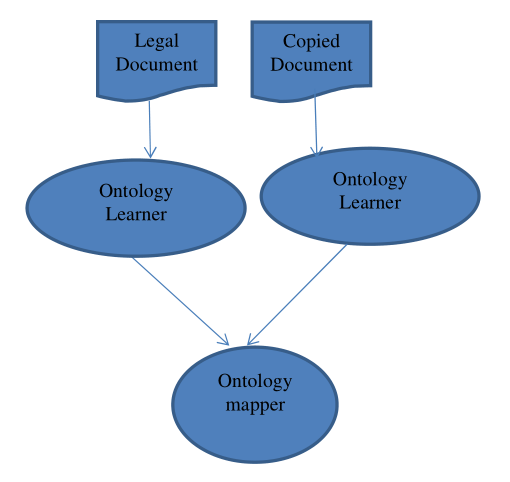
\includegraphics[scale=0.5]{ref_1_arch.png}
	\caption{Architecture of the proposed detection system.}
\end{figure}

\break

\section{Reference 8: An ontology-based retrieval system using semantic indexing}

This Masters thesis, can be divided into three parts. In chapter 2, Background information,
the authors discuss general information science with an emphasis on information retrieval (IR).
They also discuss optimizing the information retrieval or searching process implementing indexing,
ranking etc. They also discusss evaluation metrices. Finally the concept of Semantic Web is 
introduced and the application to improve IR is discussed. \\

In chapter 3, various approaches including traditional, semantic approaches are discussed. 
The authors discuss semantic indexing and their proposed models. \\

In chapter 4, the authors conceptualize their own semantic retrieval process. 

\begin{figure}[h]
	\label{ref_8_design}
	\centering 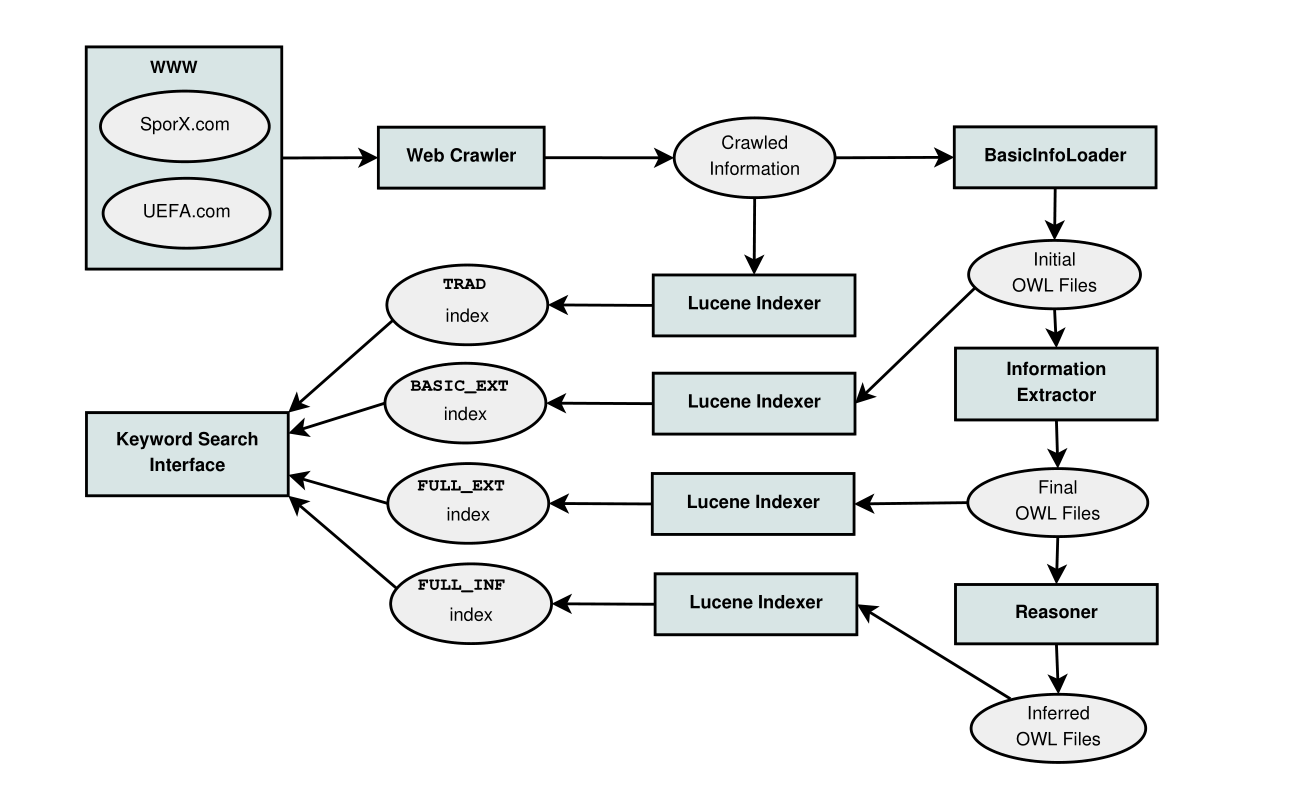
\includegraphics[scale=1.5]{ref_8_design.png}
	\caption{System design of the proposed semantic retrieval system system.}
\end{figure}

\break

So, in this system, information is gathered from \url{www.uefa.com} and \url{www.sporx.com} which
are not semantically readable. These information are then fed into  Lucene Indexer and owl ontologies are formed from the gathered xml. In this way, both a indexed search engine and semantically 
vaiable Knowledge base is created which are interlinked. Semantic ruleset is created and a 
reasoner is used. So, information can be looked up efficently and accurately.

\section{Reference 10: Towards Efficient SPARQL Query Processing on RDF Data}

In this original research paper, the authors talk about SPARQL query optimiztion. The main claims
of the authors are, in some RDF data storage systems (eg. APACHE Jena, SOR), SPARQL queries are often translated into SQL statements. But as SPARQL triples does not translate well enough into SQL statements, many self-joins and table joins are required which causes slow-downs.

\section{Reference 14: Visualizing search results and document collections using topic maps}


\chapter{Analyis of Citations of Given Paper}

\chapter{Future Work}

\begin{thebibliography}{9}
	\bibitem{latexcompanion} 
	Michel Goossens, Frank Mittelbach, and Alexander Samarin. 
	\textit{The \LaTeX\ Companion}. 
	Addison-Wesley, Reading, Massachusetts, 1993.
\end{thebibliography}

\chapter{Appendix}

\end{document}
